\section{Evaluation Metrics}
In this section, the performance of the models is analyzed through the graphs of the main evaluation metrics: ROUGE \cite{lin-2004-rouge}, WER \cite{roy2021semanticwerunifiedmetricevaluation}, cosine similarity, and BERT score \cite{zhang2020bertscoreevaluatingtextgeneration}.\\
Additionally, a custom metric \texttt{myevaluation} was also used, which will be discussed later.\\
These metrics were chosen to accurately measure the quality of the generated summaries by comparing them with the reference summaries.\\
The evaluations were conducted using the test dataset, which was not used during the model training phase.\\

\subsection{Evaluation by Permutation}
For each permutation of architectures and their respective hyperparameters,
a structured evaluation process was followed at the end of the
training phase. Below are the evaluation metrics used.

\subsection{ROUGE (Recall-Oriented Understudy for Gisting Evaluation)}
Three variants of ROUGE were calculated:
\begin{itemize}
    \item ROUGE-1: compares unigrams between the generated summary and the reference summary
    \item ROUGE-2: considers bigrams to evaluate the similarity between the two texts
    \item ROUGE-L: compares the longest common subsequence between the two texts
\end{itemize}

The graphs in Figure \ref{fig:rouge_comparison} compare the performance in terms of ROUGE-1, ROUGE-2, and ROUGE-L for the four models. The Seq2SeqBiLSTM model shows an improvement in ROUGE scores compared to Seq2SeqLSTM, Seq2Seq3BiLSTM, and Seq2SeqGRU, indicating a greater ability to capture lexical similarities.
\begin{figure}[H]
    \centering
    \rougeonesubimg{0.45}{Seq2SeqLSTM}{rouge1_seq2seq_lstm}
    \hfill
    \rougeonesubimg{0.45}{Seq2SeqBiLSTM}{rouge1_seq2seq_bilstm}
    \hfill
    \rougeonesubimg{0.45}{Seq2Seq3BiLSTM}{rouge1_seq2seq_3bilstm}
    \hfill
    %\rougeonesubimg{0.45}{Seq2SeqLSTMGlove}{rouge1_seq2seq_lstm_glove}
    %\hfill
    \rougeonesubimg{0.45}{Seq2SeqGRU}{rouge1_seq2seq_gru}
    \hfill

    \rougetwosubimg{0.45}{Seq2SeqLSTM}{rouge2_seq2seq_lstm}
    \hfill
    \rougetwosubimg{0.45}{Seq2SeqBiLSTM}{rouge2_seq2seq_bilstm}
    \hfill
    \rougetwosubimg{0.45}{Seq2Seq3BiLSTM}{rouge2_seq2seq_3bilstm}
    \hfill
    %\rougetwosubimg{0.45}{Seq2SeqLSTMGlove}{rouge2_seq2seq_lstm_glove}
    %\hfill
    \rougetwosubimg{0.45}{Seq2SeqGRU}{rouge2_seq2seq_gru}
    \hfill

    \rougelubimg{0.45}{Seq2SeqLSTM}{rougeL_seq2seq_lstm}
    \hfill
    \rougelubimg{0.45}{Seq2SeqBiLSTM}{rougeL_seq2seq_bilstm}
    \hfill
    \rougelubimg{0.45}{Seq2Seq3BiLSTM}{rougeL_seq2seq_3bilstm}
    \hfill
    %\rougelubimg{0.45}{Seq2SeqLSTMGlove}{rougeL_seq2seq_lstm_glove}
    %\hfill
    \rougelubimg{0.45}{Seq2SeqGRU}{rougeL_seq2seq_gru}
    \hfill

    \caption{ROUGE scores comparison between Seq2SeqLSTM, Seq2SeqBiLSTM, Seq2Seq3BiLSTM and Seq2SeqGRU architectures.}
    \label{fig:rouge_comparison}
\end{figure}

\subsection{WER (Word Error Rate)}
The WER is a metric that calculates the error rate between two sequences of words.\\
In particular, the WER calculates the number of insertion, deletion, and substitution operations needed to transform one word sequence into another.\\

The WER comparison, shown in Figure \ref{fig:wer_comparison}, highlights that the Seq2Seq3BiLSTM model achieves better results, indicating a greater accuracy in word generation, although the difference with the Seq2SeqBiLSTM architecture is not significant.\\

\begin{figure}[H]
    \centering
    \wersubimg{0.45}{Seq2SeqLSTM}{wer_seq2seq_lstm}
    \hfill
    \wersubimg{0.45}{Seq2SeqBiLSTM}{wer_seq2seq_bilstm}
    \hfill
    \wersubimg{0.45}{Seq2Seq3BiLSTM}{wer_seq2seq_3bilstm}
    \hfill
    %\wersubimg{0.45}{Seq2SeqLSTMGlove}{wer_seq2seq_lstm_glove}
    %\hfill
    \wersubimg{0.45}{Seq2SeqGRU}{wer_seq2seq_gru}

    \caption{WER scores comparison between Seq2SeqLSTM, Seq2SeqBiLSTM, Seq2Seq3BiLSTM and Seq2SeqGRU architectures.}
    \label{fig:wer_comparison}
\end{figure}


\subsection{Cosine Similarity}
Cosine similarity is a metric that calculates the similarity between two vectors in a multidimensional space.\\
In the specific case of summary generation, cosine similarity was calculated between the embedding vectors of the words in the generated summaries and those in the reference summaries, in order to evaluate the quality of the generated summaries.\\
Figure \ref{fig:cosine_similarity_comparison} compares the cosine similarity values. Again, the Seq2SeqBiLSTM model achieves higher values, suggesting a greater semantic correlation with the reference summaries.

\begin{figure}[H]
    \centering
    \cssubimg{0.45}{Seq2SeqLSTM}{cs_seq2seq_lstm}
    \hfill
    \cssubimg{0.45}{Seq2SeqBiLSTM}{cs_seq2seq_bilstm}
    \hfill
    \cssubimg{0.45}{Seq2Seq3BiLSTM}{cs_seq2seq_3bilstm}
    \hfill
    %\cssubimg{0.45}{Seq2SeqLSTMGlove}{cs_seq2seq_lstm_glove}
    %\hfill
    \cssubimg{0.45}{Seq2SeqGRU}{cs_seq2seq_gru}

    \caption{Cosine similarity scores comparison between Seq2SeqLSTM, Seq2SeqBiLSTM, Seq2Seq3BiLSTM and Seq2SeqGRU architectures.}
    \label{fig:cosine_similarity_comparison}
\end{figure}

\subsection{BERT Score}
BERT score is a metric that uses the BERT model to calculate the similarity between two texts.\\
In particular, BERT score calculates the similarity between the embedding vectors of the words in the generated summaries and those in the reference summaries, taking into account the semantic context of the words.\\
Figure \ref{fig:bert_score_comparison} shows the BERT score values for the different models. Again, the Seq2SeqBiLSTM model achieves better results, suggesting a greater ability to capture the semantic similarity between the generated summaries and the reference ones.

\begin{figure}[H]
    \centering
    \bertsubimg{0.45}{Seq2SeqLSTM}{bert_seq2seq_lstm}
    \hfill
    \bertsubimg{0.45}{Seq2SeqBiLSTM}{bert_seq2seq_bilstm}
    \hfill
    \bertsubimg{0.45}{Seq2Seq3BiLSTM}{bert_seq2seq_3bilstm}
    \hfill
    %\bertsubimg{0.45}{Seq2SeqLSTMGlove}{bert_seq2seq_lstm_glove}
    %\hfill
    \bertsubimg{0.45}{Seq2SeqGRU}{bert_seq2seq_gru}
    \hfill

    \caption{BERT score comparison between Seq2SeqLSTM, Seq2SeqBiLSTM, Seq2Seq3BiLSTM and Seq2SeqGRU architectures.}
    \label{fig:bert_score_comparison}
\end{figure}

\subsection{My Evaluation}
The \texttt{myevaluation} metric was designed to evaluate the quality of the generated summaries in a more detailed way.\\
It takes into account several factors, each of which has a specific weight based on its importance.\\
The formula used to calculate the \texttt{myevaluation} metric is as follows:
\[
    \texttt{MyEval} = cs\_PS\_OS \cdot W_{cs\_PS\_OS} + keyword\_overlap \cdot W_{keyword\_overlap} + bert\_score \cdot W_{bert\_score}
\]
Where:
\begin{itemize}
    \item $cs\_PS\_OS$ is the cosine similarity between the generated summary and the original one
    \item $keyword\_overlap$ is the percentage of keywords present in the generated summary compared to those in the original summary
    \item $bert\_score$ is the BERT score between the generated summary and the original one
    \item $W_{cs\_PS\_OS}$, $W_{keyword\_overlap}$ and $W_{bert\_score}$ are the weights associated with each factor
          \begin{itemize}
              \item $W_{cs\_PS\_OS} = 0.07$
              \item $W_{keyword\_overlap} = 0.03$
              \item $W_{bert\_score} = 0.9$
          \end{itemize}
\end{itemize}

Figure \ref{fig:myevaluation_comparison} shows the results of the \texttt{myevaluation} metric for the different models.\\
The Seq2SeqBiLSTM model achieves the highest scores, suggesting a superior quality of the generated summaries compared to the other models.
\begin{figure}[H]
    \centering
    \myevalsubimg{0.45}{Seq2SeqLSTM}{myeval_seq2seq_lstm}
    \hfill
    \myevalsubimg{0.45}{Seq2SeqBiLSTM}{myeval_seq2seq_bilstm}
    \hfill
    \myevalsubimg{0.45}{Seq2Seq3BiLSTM}{myeval_seq2seq_3bilstm}
    \hfill
    %\myevalsubimg{0.45}{Seq2SeqLSTMGlove}{myeval_seq2seq_lstm_glove}
    %\hfill
    \myevalsubimg{0.45}{Seq2SeqGRU}{myeval_seq2seq_gru}
    \hfill

    \caption{Comparison of the \texttt{myevaluation} metric between Seq2SeqLSTM, Seq2SeqBiLSTM, Seq2Seq3BiLSTM and Seq2SeqGRU architectures.}
    \label{fig:myevaluation_comparison}
\end{figure}

\subsection{Architectures Comparison}
Below is a comparative table (Figure \ref{fig:models_comparison_instances}) between the various implemented models, with their respective results obtained at the end of training.\\
For each model class, numerous attempts and tests were conducted, which are reported later in a comparative table of the various configuration instances and the results obtained.\\
We can immediately see that the Seq2SeqBiLSTM model achieved the best results in almost all metrics.
\begin{figure}[H]
    \centering
    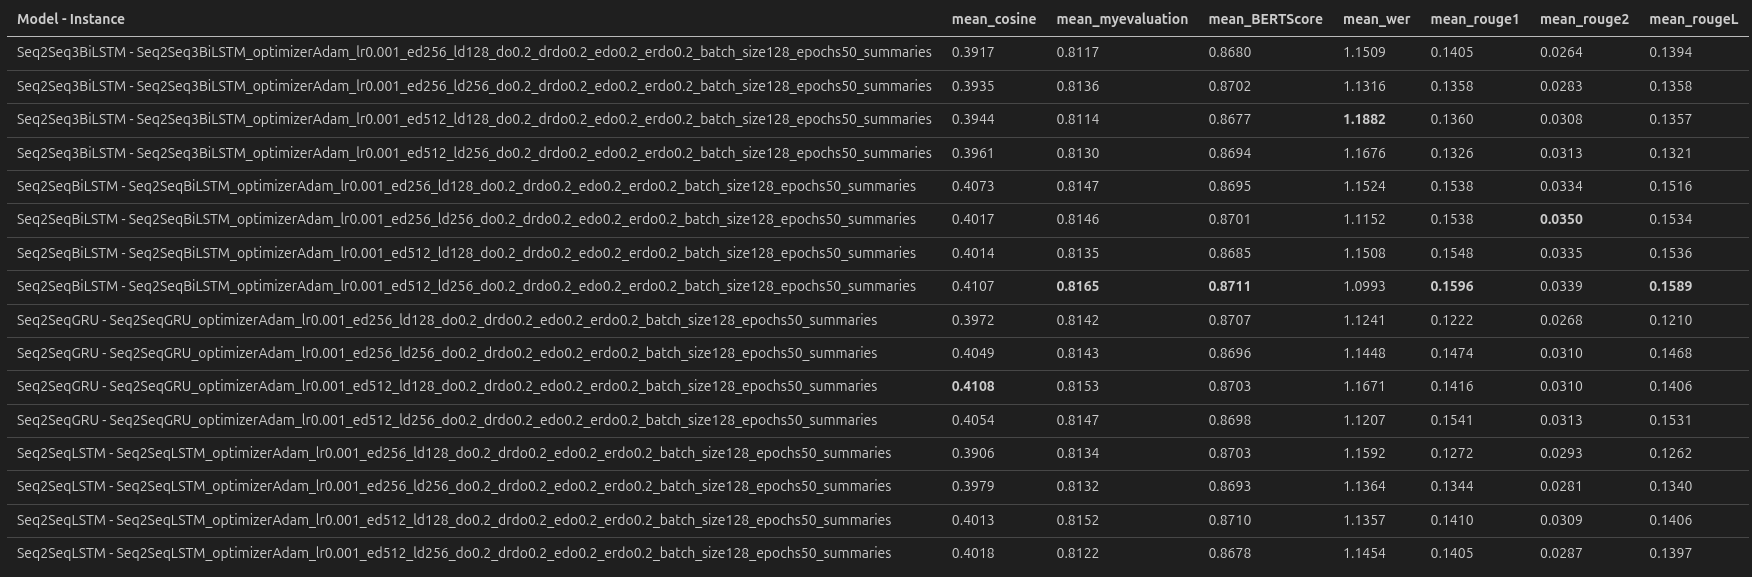
\includegraphics[width=1\textwidth]{media/models_comparison_instances.png}
    \caption{Comparative analysis of model instances}
    \label{fig:models_comparison_instances}
\end{figure}

